%
% File: chap01.tex
% Author: Liam O'Shea
% Description: Introduction chapter where the boxing goes.
%
\let\textcircled=\pgftextcircled
\chapter{My Approach}
\label{chap:intro}

\initial{T}his chapter will discuss each step of the implementation stage such as the collection of skeleton data and it's associated data format, dimensionality reduction techniques with a comparison of their suitability for this research, punch segmentation algorithms, punch classification and finally qualiy assesment.
%=======

\section{Data collection}
Once I had submitted my study to the University Ethics Committee, I visited `Bristol Boxing Gym' and `Broad Plain Boys Club' to record punch sequences from a variety of different experience levels and body types. In some cases I instructed the participants to try to throw the punches as precisely as possible, paying attention to good form. In others I asked them to make intentional beginner mistakes, such as allowing the left elbow to stick out when throwing the jab. I also asked the participants to try to keep their punches evenly spaced out when throwing them and to stand in approximately the same location as each other.

Skeletal data is recorded using the Kinect and stored as a space separated text file, with each line corresponding to one timeframe. The structure of a line is: 
$$trackingflag\;x_0\;y_0\;z_0\;\;\;trackingflag\;x_1\;y_1\;z_1\;.\;.\;.\;\;trackingflag\;x_{19}\;y_{19}\;z_{19}$$
where $x_i,y_i,z_i$ are the x,y,z coordinates representing the position of the ith joint.
A large value that could not be a Kinect measurement is used as a flag to signify the beginning of a newline. The tracking_flag is an integer which describes the status of the joint:\newline
Joint not tracked = 0, Joint position inferred = 1, Join position tracked = 2.\newline
If the joint is not tracked the position is set to (-10000, -10000, -10000) and is not used. All joint's positions are measured relative to the camera, which is considered to be at position (0,0,0).

\begin{center}
    \begin{tabular}{| l | l |}
    \hline
    Joint Number & Joint Name \\ \hline
    0 & NUI_SKELETON_POSITION_HIP_CENTER \\ \hline
    1 & NUI_SKELETON_POSITION_SPINE\\ \hline
    2 & NUI_SKELETON_POSITION_SHOULDER_CENTER\\ \hline
    3 & NUI_SKELETON_POSITION_HEAD\\ \hline
    4 & NUI_SKELETON_POSITION_SHOULDER_LEFT\\ \hline
    5 & NUI_SKELETON_POSITION_ELBOW_LEFT\\ \hline
    6 & NUI_SKELETON_POSITION_WRIST_LEFT\\ \hline
    7 & NUI_SKELETON_POSITION_HAND_LEFT\\ \hline
    8 & NUI_SKELETON_POSITION_SHOULDER_RIGHT\\ \hline
    9 & NUI_SKELETON_POSITION_ELBOW_RIGHT\\ \hline
    10 & NUI_SKELETON_POSITION_WRIST_RIGHT\\ \hline
    11 & NUI_SKELETON_POSITION_HAND_RIGHT\\ \hline
    12 & NUI_SKELETON_POSITION_HIP_LEFT\\ \hline
    13 & NUI_SKELETON_POSITION_KNEE_LEFT\\ \hline
    14 & NUI_SKELETON_POSITION_ANKLE_LEFT\\ \hline
    15 & NUI_SKELETON_POSITION_FOOT_LEFT\\ \hline
    16 & NUI_SKELETON_POSITION_HIP_RIGHT\\ \hline
    17 & NUI_SKELETON_POSITION_KNEE_RIGHT\\ \hline
    18 & NUI_SKELETON_POSITION_ANKLE_RIGHT\\ \hline
    19 & NUI_SKELETON_POSITION_FOOT_RIGHT\\ \hline
    \hline
    \end{tabular}
\end{center}

\section{Exploring Hand Movement \& Periodicity}
My first step was to organise the data in such a way that it could be usefully visualised so that I could comprehend the nature of the data that needed to be processed. I began by recording a sequence of 5 jabs, being careful to evenly time the punches before manually isolating the left wrist joint over time. In this instance the timing was important as my aim was to produce a sinusoidal-like sequence with five full `cycles' demonstrating the movement of the left hand over time {\bf Fig 3.1}.\newline
This result was promising since I could now confirm that punches could be represented by a periodic sequence. As a proof of concept isolating a single joint was a sensible first step however this cannot be reliably used to perform action recognition since it would be a single point of failure.  
If for example the joint was obscured or the Kinect mis-tracked the joint you would lose the ability to recognise an action. Since a boxing punch is based on the transference of weight and the rotation of the hip the whole pose must be considered to ensure other periodic aspects are not missed.
The use of dimensionality reduction offers increased robustness against these types of problem since it allows the entire skeleton to be represented in low dimensionality data and as such will not be as sensitive to noise or failures to track. 

\begin{figure}[h]
    \centering
    \includegraphics[height=0.25\textheight]{fig04/lwrist.pdf}
    \mycaption[Position of the left wrist over time]{Left wrist joint's movement in the z direction over time. The x-axis represents time (kinect frames) and the y-axis the distance of the fist from the Kinect}
\end{figure}

\section{Pose Representation}
Next I needed to find a meaningful way of visualising the entire skeleton over time, so that the pose as a whole could be be represented and assessed. I na{\"i}ively began by plotting the entire data set, which produced a reasonably jagged signal with two troughs followed by a large peak before levelling of again. {\bf Fig 3.7 (a)}. At this point I realised attempting to plot the skeleton data in this way would not be useful, but as a test I differentiated the raw data to produce a velocity as opposed to distance. My hope was that since velocity is position invariant it would be a better choice than using the raw co-ordinates. Unfortunately I found that the velocity introduced more noise and due to this it was clear that it was going to be much more difficult to segment later on.

Realising that for now I needed to look at individual joints I took the left write joint and plotted its movement in the z direction over time as well as plotting the differential of that to give me the velocity. As you can see from {\bf Fig 3.7 (b)}, the velocity data was much more useful and produced a reasonably smooth periodic sequence. Since the initial recording was 10 jabs one after the other I expected a periodic, cyclical signal to be produced.

Since PCA was a familiar method I implemented it in Matlab using three principal components and plotted the first projection coefficient for the first principal component with both the distance and velocity data. From this we can see that the distance data was slightly jagged with a local maxima which might obstruct attempts to automatically segment punches. The velocity data produced a smoother series but introduced unwanted noise towards the beginning and end of a sequence. {\bf Fig 3.2}

Next I plotted all three projection coefficients for the three principal components for both distance and velocity. {\bf (Fig 3.8)} We can see for the first projection coefficient both distance and velocity are similar, with distance being slightly more jagged at the peaks of the punching period and velocity being more jagged at the start and end.
For the second they are both fairly similar but with distance having less peaks and troughs and with only one dramatic spike at 250 as opposed to two at 50 and 275.
For the third the depth comes out ahead with a smoother signal which again has less `spikes', (which will make it easier to segment.) Although by eye it looks like the depth data under PCA produces a more useful periodic signal neither are particularly convincing so I will have to perform a more precise comparison.

\begin{figure}[h!]
\centering
\begin{minipage}{6.0cm}
    \centering
    \subtop[]{\includegraphics[height=0.25\textheight]{fig04/fig02}}
    \label{fig:1}
\end{minipage}
\hspace{2.0cm}
\begin{minipage}{6.0cm}
    \centering
    \subtop[]{\includegraphics[height=0.25\textheight]{fig04/fig03}}
    \label{fig:2}
\end{minipage}
\mycaption[Projection coefficient of a jab over time]{A plot of the projection coefficient for the first principal component for a jab over time for (a) distance, (b) velocity}
\end{figure}
------------------------------------------


\section {Dimensionality Reduction (DR) Comparison}
Each dimensionality reduction method was evaluated on its ability to produce useful, smooth and sinusoidal output to aid automatic segmentation. Automatic segmentation is a crucial step in the project, since on a larger scale much bigger data sets will need to be used and collated from multiple sources. If these can be processed and automatically segmented this will remove any manual work required and make this a truly useful system. I used the Matlab Dimensionality Toolbox and the `intrinsic_dim' function that performs an estimation of the intrinsic dimensionality of a dataset X given a specific method. This was calculated using six different methods, maximum-likelihood estimation (MLE), correlation dimension estimation (CorrDim), nearest neighbourhood, packing numbers, Geodesic minimum spanning tree (GMST) and eigenvalue estimation.
These results were then combined and averaged to produce a dimension {\bf d} to be used as an argument for LLE, Hessian LLE, Laplacian, LTSA, CCA and PCA (see background). The lower dimensionality data was then plotted and analysed.
The projection coefficient of the first principal component, plotted for multiple dimensionality reduction techniques shows that PCA gives the most useful results, followed closely by CCA. If we then look at the second projection coefficient we can see that PCA performs second to LTSA but LTSA performs poorly for the first component. Since the others prduce noisier and less sinosidal-like results it makes PCA the obvious choice. Although PCA is simpler than more modern techniques, it actually produced the most consistently smooth cyclical signal.
\begin{figure}[h!]
    \centering
    \includegraphics[height=0.25\textheight]{fig04/drcomp.pdf}
    \mycaption[Dimensionality Reduction comparison graph for PC1]{The projection coefficient for the first principal component as produced by a variety of DR techniques over time}
    \label{fig:drcomp}
\end{figure}
\begin{figure}[h!]
    \centering
    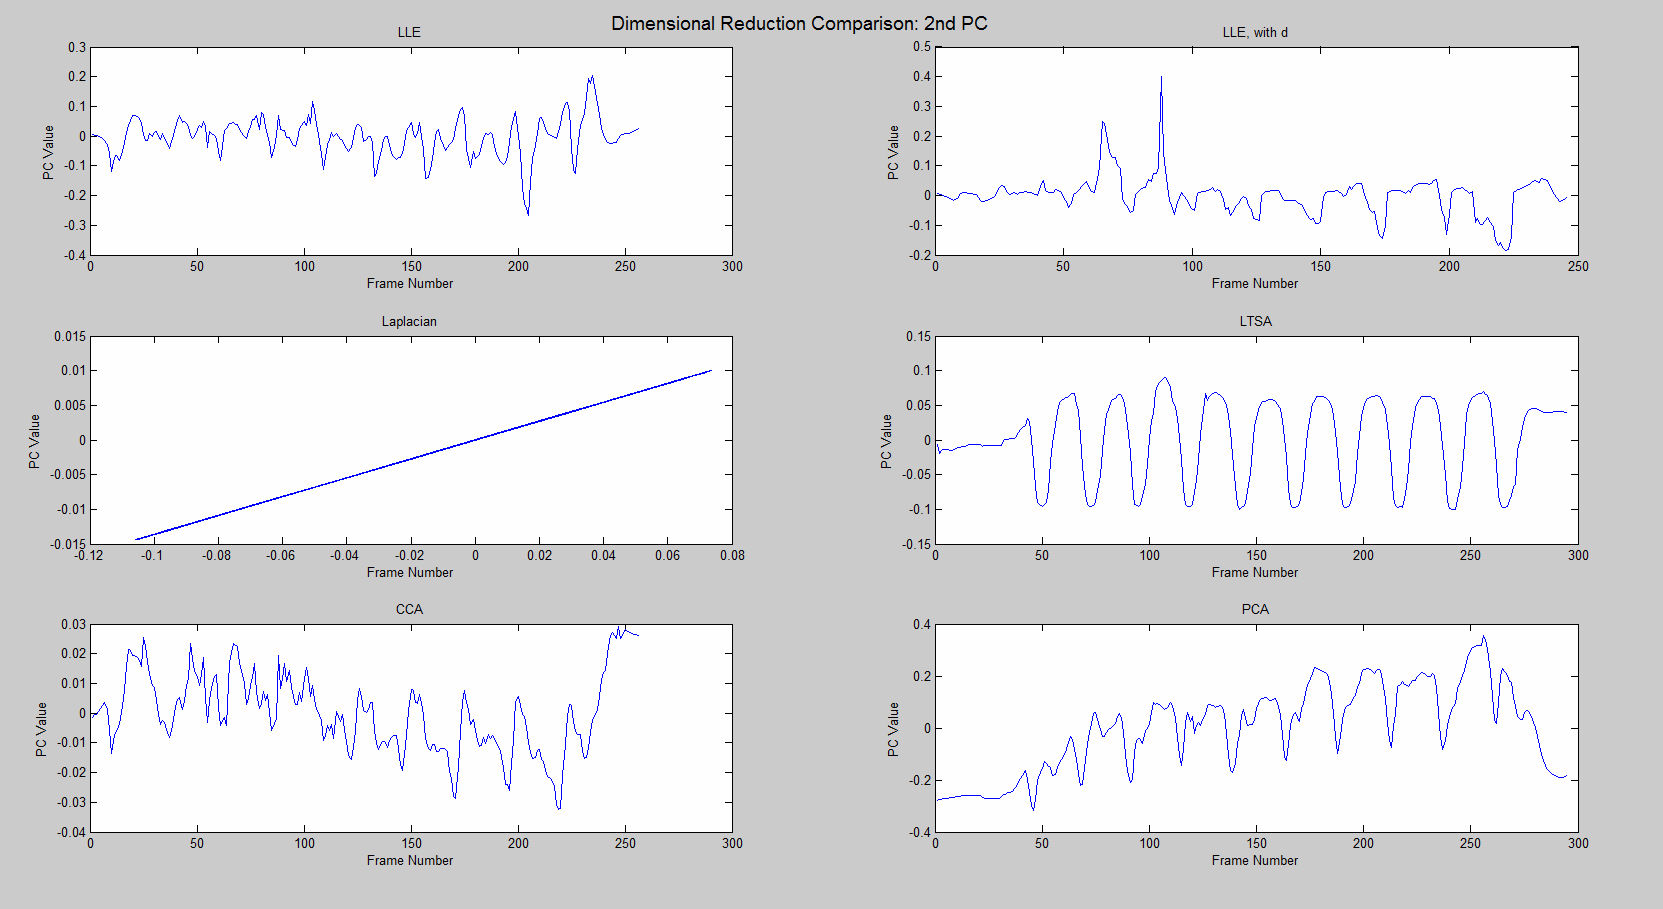
\includegraphics[height=0.25\textheight]{fig04/drcomp2.pdf}
    \mycaption[Dimensionality Reduction comparison graph for PC2]{The projection coefficient for the second principal component as produced by a variety of DR techniques over time}
    \label{fig:drcomp}
\end{figure}\clearpage


\subsection{Pose Reconstruction}
Another benefit of using PCA is that it is possible to reconstruct the original pose using the equation $$y = U*a+Xm$$ where U is the eigenvectors, a is the projection coefficients and Xm the mean of the original data. Since we are going from low dimensionality data back to high dimensionality data it is inevitable there will be some reconstruction error. However by plotting this reconstruction along with the original it is possible to visualise how closely the principal components generated represent the original {\bf Fig 3.5}. This is crucial because the decomposition can be verified to make sure that important information is not lost during the reduction process.\qquad

\section{Punch Segmentation Algorithm}
After failing to find a way to automatically segment punches using existing methods it became apparent that a custom algorithm will be needed for this task, which can be broken down into several steps.

\begin{enumerate}[noitemsep]
  \item Perform PCA on raw data.
  \item Smooth the principal coefficients.
  \item Find the local maxima and minima of the first principal coefficient.
  \item Remove erroneous minima/maxima using heuristic rules.
  \item Take a number of evenly spaced samples from between two maximum points.
  \item Fetch the unsmoothed PCA data that corresponds to the time the samples were taken.
  \item Train classifier on new data.
\end{enumerate}
Each frame representing 20 joint positions is reduced from 60 dimensions to 6 principal coefficients per frame. Next the principal coefficients are smoothed to remove any `wrong' minima/maxima which would prevent the automated segmentation of punches. All remaining maxima are then passed through a set of heuristic rules, that checks the location of a maxima point relative to its neighbourhood points, to determine if it is legitimately the start of a punch. Once this has been achieved a number of evenly spaced samples are taken from between two maximum points resulting in each individual punch being sampled. As the sequence is temporal each sample relates to a time which is then used to fetch the unsmoothed principal coefficients at that time. It is necessary to use the unsmoothed data for classification since this data has been overly-smoothed as its purpose was segmentation. As a result the unique shape and characteristics of each sequence are lost and therefore it no longer accurately represents a pose. Certain elements of the pose such as the movement of the hip joint which would correspond to a rotation in the pose would be crucial to successfully classify punches. Put simply, without using the unsmoothed data the classifier would fail to find distinct features for each class of punch and so would be unable to classify effectively. {\bf Fig 3.6}


\begin{figure}[t]
 % \hspace{-1.5cm}
\begin{flushleft}
\centering
\begin{minipage}{6.0cm}
    \centering
    \subtop[]{\includegraphics[height=0.25\textheight]{fig04/rp1-crop}}
    \label{fig:a}
\end{minipage}
\hspace{2.0cm}
\begin{minipage}{6.0cm}
    \centering
    \subtop[]{\includegraphics[height=0.25\textheight]{fig04/rp2-crop}}
    \label{fig:b}
\end{minipage}
\qquad
% \centering
\begin{minipage}{6.0cm}
    \centering
    \subtop[]{\includegraphics[height=0.25\textheight]{fig04/rp3-crop}}
    \label{fig:a}
\end{minipage}
\hspace{2.0cm}
\begin{minipage}{6.0cm}
    \centering
    \subtop[]{\includegraphics[height=0.25\textheight]{fig04/rp4-crop}}
    \label{fig:b}
\end{minipage}
\qquad
\centering
\begin{minipage}{6.0cm}
    \centering
    \subtop[]{\includegraphics[height=0.25\textheight]{fig04/rp5-crop}}
    \label{fig:a}
\end{minipage}
\hspace{2.0cm}
\begin{minipage}{6.0cm}
    \centering
    \subtop[]{\includegraphics[height=0.25\textheight]{fig04/rp6-crop}}
    \label{fig:b}
\end{minipage}
\qquad
\end{flushleft}
\mycaption[Comparison of original pose \& reconstructed pose]{Each graph represents a single pose with the original data in green and the reconstructed data in red obtained from back projection. We can see from the reconstruction how much data has been lost as a result of dimensionality reduction.
{\bf(a)} Jab  {\bf(b)} Cross {\bf(c)} Left-Hook {\bf(d)} Right-Hook {\bf(e)} Left-Uppercut {\bf(f)} Right-Uppercut}
\end{figure}

\begin{figure}[h]
\hspace{-1.5cm}
\centering
\begin{minipage}{9.0cm}
    \centering
    \subtop[]{\includegraphics[height=0.40\textheight]{fig04/usr-crop.pdf}}
    \label{fig:kinect2}
\end{minipage}
% \hspace{1.0cm}
\qquad
\begin{minipage}{9.0cm}
    \centering
    \subtop[]{\includegraphics[height=0.40\textheight]{fig04/usrclose-crop}}
    \label{fig:kinect3}
\end{minipage}
\mycaption[Original \& smoothed right uppercut demonstrating feature loss]{An overlay of the original principal coefficients (red) and smoothed principal coefficient (blue) for a right uppercut. 
(a) Displayed is an entire punch sequence; notice that the smoothed sequence covers approximately $\frac{2}{3}$rds the area than that of the original, demonstrating a substantial amount of information loss.
Also notice the maxima marked on the smoothed curve correspond to peaks on the unsmoothed sequence. (b) Displayed is a closer look at the half-way point of four individual hooks. Observe the unique shape of the hooks as they increase and decrease several times as they tend to and then away from the minima. Witness the effect smoothing has on this unique characteristic, this would be a very useful feature for a classifier.}
\end{figure}

\paragraph{Heuristic Rules}
As the punch sequence is sinusoidal-like every maxima should correspond to the beginning of a punch (and the end of the previous one) so it is known that the start of every punch should fall within a certain range of amplitude. This allowed me remove a lot of false positives that had not been removed in smoothing by simply thresholding. Each type of punch has its own unique signature so a different threshold is applied depending on the punch, although there are some common rules that are applied to the left or right hand side of the body. Once this is done each maxima is looked at relative to its neighbours to try to determine if it is likely to be the beginning of a punch. I used the Pythagorean theorem to calculate the distance between a maxima and its neighbours; if the distance is too small it is clear that one of the points is erroneous and that only one of these will be necessary for segmentation. Likewise if a neighbour is too far away it becomes obvious that one of the maxima is incorrect and needs to be removed. 

\section{Classification}
Once the data has been successfully segmented and reduced I began to experiment with a range classifiers, as referenced in the background section. 


\subsection{Feature Extraction (PCA)}
Once the data has been successfully segmented into individual punches we can begin to extract features that can be used to train a classifier. Twelve to fifteen evenly spaced samples are taken for each individual punch, depending on the classifier to be used later. Each sample corresponds to a point in time which is used to extract the required number of principal coefficients for each point. Taking three coefficients as an example we would have $36 - 45$ features for each punch.
Once all the different punch sequences are sampled for each type of punch we can use this data to train a classifier. A multi-class SVM, decision tree, Random Forest and neural network were tested.

\subsection{Feature Extraction (DTW)}
After using DTW I found that there was not enough difference between the various segmented punches to give me an effective way to segment. Comparing jabs to other jabs yielded similarity values from $0 - 1.589$ with an average difference of $0.499$, comparing jabs to crosses yielded similarity values from $0-2.113$ with the average $0.716$. Due to the large spread of values across the classes and similarity in values between different classes of punche there was not enough of a consistent difference in the score to be able to extract features or have an indication of the type of punch.

\subsection{Fast Fourier Transform (FFT)}
 I investigated the possibility of running a FFT on the raw data as well as each segmented punch that was obtained from using PCA and my own segmentation algorithm. The range for the coefficients was $0 - (63.030 - 0i)$ with a spread across all of the different types of punches. Unfortunately this meant the coefficients obtained in both cases proved to be a poor differentiator between punches due to the coefficients being so variable even within the same punch types.

 \subsection{Neural Networks (NN)}
 I used NNs extensively since my initial attempts at classification, produced very promising results compared to the other classifiers, even when the punch segmentation algorithm was in development resulting in fairly noisy input. I discovered that when using between 1-3 projection coefficients the network size performed better when smaller with 10 neurons, with 5 not being able to handle the complexity of the data and 20 beginning to over-fit the data to the training set {\bf Tab 3.1}. By the end of the project when using between 5-7 eigenvectors with a large training set 25 neurons was the optimal network size.
\begin{table}[h]
\begin{center}
    \begin{tabular}{ | l | c  | c | c | c |}
    \hline
    n-neurons & 5 & 10 & 15\\ \hline
    Run 1 & 11.76\% & 11.76\% & 14.71\%\\ \hline
    Run 2 & 8.82\% & 2.94\% & 20.59\%\\ \hline
    Run 3 & 14.71\% & 20.59\% & 20.59\%\\ \hline
    Run 4 & 29.84\% & 8.82\% & 11.76\%\\ \hline
    Run 5 & 17.65\% & 5.88\% & 5.88\%\\ \hline
    \textbf{Avg} & \textbf{16.56\%} & \textbf{10.00\%} & \textbf{14.71\%}\\ \hline
    % \hline
    \end{tabular}
\mycaption [Neural Network Percentage Error]{Punch classification error of different size neural networks on a six class problem.
(Jab, Cross, Left-Hook, Right-Hook, Left-Uppercut, Right-Uppercut)}
\end{center}
\end{table}

 \subsection{Support Vector Machines (SVM)}
I tested SVM as a technique on a two-class problem, after reading about its sucess rate in my literature review and concluding that this technique worked well and was worth pursuing. Unfortunately Matlab does not support a multi-class SVM so I used LIBSVM a support vector machine library. I choose this since the end goal was to have a real-time system and this particular part was implemented in c which dramatically increased performance compared to others that were tried. 

After trying several variants of SVM, I discovered the most effective used a radial basis kernel and probability estimates to determine the class that each each input belongs to.
It also performed best on smaller data sets with ten samples (per principal coefficient) {\bf Table 3.2}. However with the larger datasets and increased number of eigenvectors used later in this project I found fifteen to be optimal.

\begin{table}[h]
\begin{center}
    \begin{tabular}{ | l | c  | c | c | c |}
    \hline
    n-samples & 5 & 10 & 15 & 20\\ \hline
    Run 1 & 88.13\% & 93.48\% & 82.43\% & 84.78\%\\ \hline
    Run 2 & 94.65\% & 95.65\% & 82.61\% & 86.96\%\\ \hline
    Run 3 & 92.48\% & 86.97\% & 97.83\% & 93.48\%\\ \hline
    Run 4 & 87.13\% & 86.96\% & 91.30\% & 84.78\%\\ \hline
    Run 5 & 90.30\% & 86.96\% & 89.13\% & 76.09\%\\ \hline
    \textbf{Avg}   & \textbf{85.74\%} & \textbf{95.65\%} & \textbf{88.60\%} & \textbf{85.20\%}\\ \hline
    % \hline
    \end{tabular}
\mycaption [SVM Classification Accuracy Testing]{Punch classification accuracy of SVM with different numbers of samples used on a six class problem using a reduced dataset (Jab, Cross, Left-Hook, Right-Hook, Left-Uppercut, Right-Uppercut)}
\end{center}
\end{table}

\begin{figure}[h!]
\centering
\begin{minipage}{6.0cm}
    \centering
    \subtop[]{\includegraphics[height=0.25\textheight]{fig04/fig06}}
    \label{fig:1}
\end{minipage}
\hspace{2.0cm}
\begin{minipage}{6.0cm}
    \centering
    \subtop[]{\includegraphics[height=0.25\textheight]{fig04/fig07}}
    \label{fig:2}
\end{minipage}
\mycaption[Pose representation using distance \& velocity]{Distance data is shown in blue and velocity data shown in green.
(a) All skeleton data has been plotted, with the x-axis corresponding to a joint co-ordinate. There are 20 joints each represented by 3 co-ordinates (x,y,z) hence the range 0-60. We can see a spike at ~40 which corresponds to joints 15 and onwards which are the right hip, right knee, right ankle and right foot. The y-axis represents distance from the Kinect in the z direction which explains the spike since in a boxing stance the right hand side of the body should be further away.
(b) Wrist joint over Time}
\end{figure}

\begin{figure}[h!]
\hspace{-1.5cm}
\centering
\begin{minipage}{6.0cm}
    \centering
    \subtop[]{\includegraphics[height=0.25\textheight]{fig04/pc1}}
    \label{fig:kinect2}
\end{minipage}
\hspace{1.0cm}
\begin{minipage}{6.0cm}
    \centering
    \subtop[]{\includegraphics[height=0.25\textheight]{fig04/pc2}}
    \label{fig:kinect3}
\end{minipage}
\qquad
\centering
\begin{minipage}{6.0cm}
    \centering
    \subtop[]{\includegraphics[height=0.25\textheight]{fig04/pc3}}
    \label{fig:kinect3}
\end{minipage}
\mycaption[Graphs of the projection coefficient for the first principal component of distance \& velocity]{The projection coefficient for the first principal component for distance data (green) and
velocity data(red).
(a) First projection coefficien tsta(b) second projection coefficient (c) third projection coefficient}
\end{figure}